\documentclass[12pt,a4paper]{article}
\usepackage[utf8]{inputenc}
\usepackage{amsmath,amssymb,amsfonts}
\usepackage{graphicx}
\usepackage{hyperref}
\usepackage{tikz}
\usepackage{listings}
\usepackage{xcolor}

\title{A \textbf{Truly} Problematic \& \textit{Perverse} Document: \texorpdfstring{$\mathcal{L}_{\text{ATEX}}$}{LATEX} Gone Wild}
\author{Dr. \texorpdfstring{$\Sigma$}{Sigma} Chaos \and Prof. $\aleph_0$ Madness}
\date{\today}

\begin{document}

\maketitle

\begin{abstract}
This document demonstrates \LaTeX{} parsing challenges: nested commands, math modes, special characters, deeply nested section hierarchies, malformed structures, and encoding nightmares. $\int_{0}^{\infty} e^{-x^2} dx = \frac{\sqrt{\pi}}{2}$ proves math works even in chaos.
\end{abstract}

\section{Introduction: The Gamma-Function Saga}
This section has \textbf{bold}, \textit{italic}, and \texttt{monospace} text mixed with math: $E = mc^2$. We also have \href{https://example.com}{hyperlinks} and \cite{fake_ref} citations.

\subsection*{Starred Subsection: Title with "Quotes" and 'Apostrophes'}
This subsection is starred and has problematic characters in its title: /\\:*?"<>|. The content includes:
\begin{itemize}
\item Item 1: $\alpha + \beta = \gamma$
\item Item 2: $\lim_{x \to \infty} \frac{1}{x} = 0$
\item Item 3: \verb|inline code with $math$|
\end{itemize}

\subsection{Subsection with Extremely Long Title That Exceeds Fifty Characters for Filename Testing and Contains More Problematic Elements}
This subsection tests filename truncation. The content includes code listings:

\begin{lstlisting}[language=Python]
def problematic_function():
    return "String with \n, \t, \\, and $math$"
\end{lstlisting}

\subsubsection{Deep Nesting Level 3: Maxwell Equations}
This is Maxwell's equation in a deeply nested subsubsection with very long math that should be handled properly.

\subsubsection*{Another Starred Deep Section with: \texorpdfstring{$\oint_{\partial S} \mathbf{B} \cdot d\mathbf{l} = \mu_0 I_{\text{enc}}$}{Integral Formulation}}
More complex physics math here.

\section{Methods: Advanced \LaTeX{} Techniques}
This section contains tables, figures, and more complex structures.

\begin{table}[h]
\centering
\begin{tabular}{|c|c|c|}
\hline
\textbf{Symbol} & \textbf{Name} & \textbf{Value} \\
\hline
$\pi$ & Pi & 3.14159... \\
$e$ & Euler's number & 2.71828... \\
$\phi$ & Golden ratio & 1.61803... \\
\hline
\end{tabular}
\caption{Mathematical constants}
\end{table}

\subsection{TikZ Graphics}
Here's some TikZ code that might break parsers:

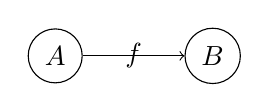
\begin{tikzpicture}
\node[circle,draw] (A) at (0,0) {$A$};
\node[circle,draw] (B) at (2,0) {$B$};
\draw[->] (A) -- (B) node[midway] {$f$};
\end{tikzpicture}

\subsubsection{Nested Math and Commands: Integral Formulations}
More challenging content here.

\section{Results: File Paths Like C:\textbackslash Windows\textbackslash System32\textbackslash problematic.exe}
This section title contains Windows-style paths and backslashes that should be sanitized.

\subsection{Empty Content Subsection}
This subsection has no content after the header.

\subsubsection{Subsubsection with Only Math}
$\sum_{n=1}^{\infty} \frac{1}{n^2} = \frac{\pi^2}{6}$

\section{Conclusion: Final Thoughts on R-n Spaces}
This concludes our perverse document. The bibliography follows.

\begin{thebibliography}{9}
\bibitem{fake_ref}
Chaos, A.S. (2023). \emph{Perverse \LaTeX{} Documents}. Journal of Problematic Parsing, 42(3), 1-100.

\bibitem{math_ref}
Madness, P.E. (2024). \emph{Mathematical Typography Gone Wrong}. International Conference on Document Chaos.
\end{thebibliography}

\end{document}